\documentclass[12pt]{article}
\usepackage[a4paper, left=3cm, right=3cm]{geometry}
\usepackage{pgfplots}
\pgfplotsset{compat=1.17}

\title{Relatório 3º projeto ASA 2023/2024}
\author{Grupo: TP048 \\ Aluno: Gabriel Silva (102637)}
\date{}

\begin{document}
\maketitle

\section{Descrição do Problema e da Solução}

\subsection{Descrição do Problema}
O problema abordado neste projeto está na otimização da produção e venda de brinquedos no Natal para a empresa UbiquityInc. Dado um conjunto de brinquedos individuais e pacotes especiais, que contêm três brinquedos individuais, queremos determinar qual o lucro máximo que se pode obter diariamente, tendo em conta o limite máximo de produção de cada brinquedo individual e a quantidade máxima total de brinquedos que podem ser produzidos por dia.

\subsection{Descrição da Solução}
Para resolver este problema de otimização, um modelo de programação linear foi desenvolvido usando a biblioteca PuLP em Python. O objetivo é estimar o lucro máximo que a UbiquityInc pode obter diariamente, considerando as restrições de produção e a introdução de pacotes especiais.

\begin{itemize}
    \item Variáveis do problema:
        \begin{itemize}
            \item $x(i)$: quantidade de brinquedos individuais do tipo $i$ a serem produzidos.
            \item $y(i, j, k)$: quantidade de pacotes especiais que contêm os brinquedos \{i, j, k\}, a serem produzidos.
        \end{itemize}
    \item Especificação do problema linear: O programa linear visa maximizar o lucro total, considerando os lucros de brinquedos individuais e pacotes especiais, sujeitos a diversas restrições. O programa inclui os seguintes componentes:
        \begin{itemize}
            \item Função Objetivo: Maximizar $\sum{l(i) \cdot x(i)} + \sum{l(i,j,k) \cdot y(i,j,k)}$
            \item Restrições:
                \begin{itemize}
                    \item A quantidade de brinquedos individuais do tipo $i$ a serem produzidos não deve exceder a capacidade de produção do brinquedo: $x(i) \leq c(i)$.
                    \item A quantidade de pacotes especiais que contêm os brinquedos \{i, j, k\} a serem produzidos não deve exceder a menor capacidade de produção do brinquedo dos brinquedos que constituem o pacote: $y(i) \leq \min\{c(i), c(j), c(k)\}$.
                    \item A quantidade total de produção de brinquedo não deve exceder a quantidade máxima de produção diária: $\sum{x(i)} + \sum{3 \cdot y(i,j,k)} \leq \text{max}$.
                \end{itemize}
        \end{itemize}
\end{itemize}

\section{Análise Teórica}

A complexidade do programa linear depende dos parâmetros do problema, especificamente do número de brinquedos ($n$) e do número de pacotes ($p$).

\begin{itemize}
    \item O número de variáveis no programa linear é $O(n+3p)$, onde $n$ representa brinquedos individuais e $3p$ representa pacotes especiais.
    \item O número de restrições no programa linear é $O(n+p)$, considerando restrições para produção individual de brinquedos, produção de pacotes especiais e o limite total de brinquedos.
\end{itemize}

\section{Análise Experimental}

\begin{figure}[ht]
    \centering
    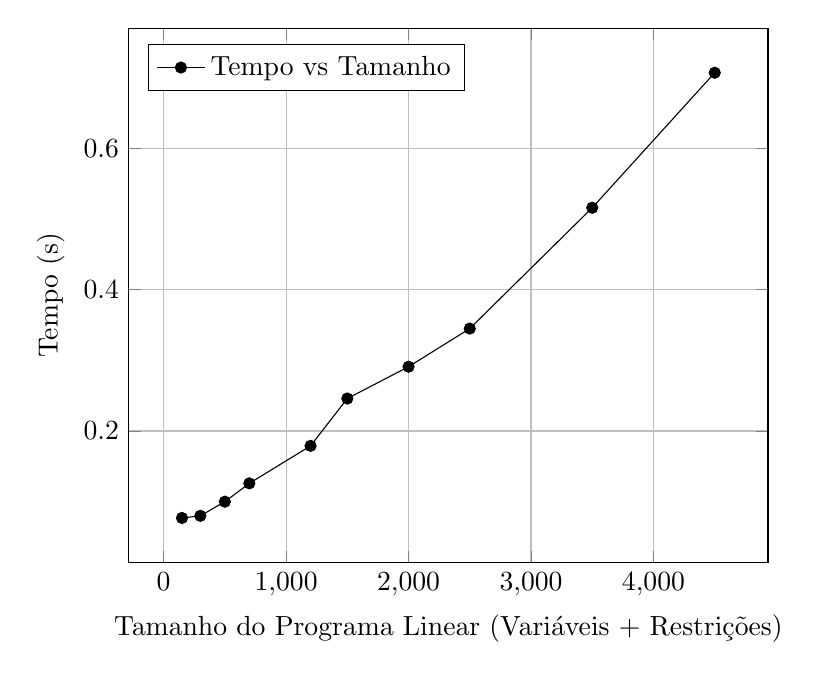
\begin{tikzpicture}
        \begin{axis}[
            xlabel={Tamanho do Programa Linear (Variáveis + Restrições)},
            ylabel={Tempo (s)},
            legend pos=north west,
            grid=both,
            width=0.8\textwidth,
        ]
        
        \addplot[mark=*] coordinates {
            (150, 0.077)
            (300, 0.080)
            (500, 0.100)
            (700, 0.126)
            (1200, 0.179)
            (1500, 0.246)
            (2000, 0.291)
            (2500, 0.345)
            (3500, 0.516)
            (4500, 0.707)
        };

        \legend{Tempo vs Tamanho}
        \end{axis}
    \end{tikzpicture}
    \caption{Tempo de Execução em Função do Tamanho do Programa Linear}
    \label{fig:experimental_graph}
\end{figure}

\end{document}